% Figure 1, traced from the original printed diagram on page 12.
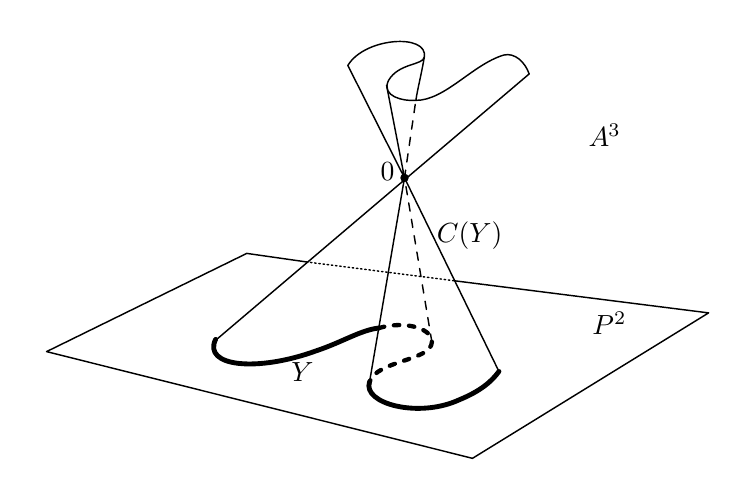
\begin{tikzpicture}[x=.34bp,y=-.34bp,line width=.52bp,line cap=round,line join=round]
  \path[use as bounding box] (0,0) rectangle (735,468);
  % The projective plane, with the far edge hidden by the cone.
  \draw (295,248)--(232,239)--(20,343)--(471,456)--(721,302)--(452,268);
  \draw[densely dotted] (295,248)--(452,268);
  % Generators and the upper cross-section.
  \draw (199,331)--(531,49)
        (339,40)--(399,159)--(499,364)
        (362,375)--(399,159)--(380,61);
  \draw[dashed] (428,333)--(399,159)--(411,77);
  \draw (339,40) .. controls (357,10) and (424,6) .. (420,31)
                 .. controls (419,40) and (393,37) .. (382,56)
                 .. controls (374,73) and (398,78) .. (411,77)
                 .. controls (442,77) and (471,39) .. (504,29)
                 .. controls (516,26) and (527,37) .. (531,49)
        (420,31) .. controls (417,49) and (413,64) .. (411,77);
  % The two visible arcs and the hidden arc of Y.
  \draw[line width=1.75bp] (199,330) .. controls (185,359) and (243,365) .. (306,342)
    .. controls (333,333) and (353,320) .. (372,318);
  \draw[line width=1.75bp] (362,375) .. controls (354,398) and (414,414) .. (457,394)
    .. controls (479,385) and (491,375) .. (499,364);
  \draw[line width=1.55bp,dash pattern=on 1.95bp off 3.5bp] (372,318)
    .. controls (404,309) and (430,321) .. (428,333)
    .. controls (427,353) and (370,352) .. (362,375);
  \fill (399,159) circle[radius=1.52bp];
  \node[inner sep=0pt] at (381,152) {$0$};
  \node[inner sep=0pt] at (468,220) {$C(Y)$};
  \node[inner sep=0pt] at (291,365) {$Y$};
  \node[inner sep=0pt] at (611,114) {$\mathbb{A}^{\mkern-.8mu 3}$};
  \node[inner sep=0pt] at (616,313) {$\mathbb{P}^{2}$};
\end{tikzpicture}
